\documentclass{article}
\usepackage[utf8]{inputenc}
\usepackage{amsmath}
\usepackage{amssymb}
\usepackage[nottoc]{tocbibind}
\usepackage{parskip}
\usepackage{amsthm}
\usepackage{hyperref}
\usepackage{enumitem}
\usepackage{tikz}
\usetikzlibrary{graphs}

\title{CMSC351: Prerequisite}
\author{Johning To}
\date{5/23/2023}

\renewcommand{\contentsname}{}

\begin{document}
\maketitle

\tableofcontents
\clearpage

\section{Symbols}
\begin{enumerate}
  \item For all ($ \forall $)
  \item There exists ($ \exists $)
  \item Element in set ($ \in $)
  \item Greater than ($ > $)
  \item Less than ($ < $)
  \item Greater than equal ($ \ge $)
  \item Less than equal ($ \le $)
\end{enumerate}

\clearpage

\section{Proofs}
\subsection {Weak Induction}
First, we need to prove $ \forall n \ge n_0 $ $ P(n) $ we first prove $ P(n_0) $ (which is the base case) and
then we prove $ \forall k \ge n_0 \; P(k) \rightarrow P(k+1) $ (which is the inductive step) (you can also prove $ P(k - 1) $).
The assumption of $ P(k) $ in the inductive step is the inductive hypothesis.

Ultimately, for the inductive step we are trying to find that for any $ k \ge n_0 $ if $ P(k) $ is true, then $ P(k + 1) $ is also true. 

\textbf{Example:}
Suppose we have a set of nested Russian dolls (Matryoshka dolls). Each doll is contained with another doll, each doll is labeled 1, 2, 3 and so on. 

In this hypothetical, there are two things that are true. Let's say $ M(n) $ is true iff (if and only if) doll $ n $ has another doll contained.
\begin{enumerate}[label=(\alph*)]
\item The first doll has another doll contained. That is, $ M(n) $ is true.

\item For every doll k, if doll k has another doll inside then doll $ k + 1 $ has another doll inside.
\end{enumerate}
$$ \forall k \ge 1, M(k) \rightarrow M(k + 1) $$

We can now conclude that $ \forall n \ge 1, M(n) $.

\subsection {Strong Induction}
The goal of strong induction is we need to find some property, we can say $ P(n) $ and 
we need to find some n greater than equal to a ($ n \ge a $).

How can we accomplish this?

\textbf {Step 1 (Basis step):} We are going to prove for $ P(a) $ (we would just prove $ P(a) $ for weak induction), $ P(a + 1) $, ...,
for some finite number say $ P(b) $. 

($P(a),\; P(a + b),\;...,\;P(b)$) $ \leftarrow $ we prove each of these.

\textbf {Step 2 (Induction):} We can now assume $ P(i) $ where $ a \le i \le k $. (Assume $ P(i) $).
Then, we prove $ P(k + 1) $.

\textbf {Example: Fibonacci Sequence}
\begin{proof}
Claim: The Fibonacci Sequence is defined as the following: $ F(0) = 0, F(1) = 1 $ and for $ n \ge 2, F(n) = F(n - 1) + F(n - 2). $
We want to prove that for all $ n \ge 0 , F(n) \le 2^n $

Base cases:
\begin{alignat*}{2}
For\; n = 0: F(0) = 0 \le 2^0 = 1
\\
For\; n = 1: F(1) = 1 \le 2^1 = 1
\end{alignat*}
For both these base case, they hold true. 

Inductive Step: 
Assume that for all $ i $, $ 0 \le i \le k $, we have $ F(k) \le 2 ^ k $.

(This could also be known as the inductive hypothesis)

We now need to prove $ F(k + 1) \le 2 ^ {k + 1} $.

By the inductive hypothesis, we have $ F(n) \le 2^n $ and $ F(n - 1) \le 2^{n-1} $.

We can prove by which:
\begin{center}
  $\begin{aligned}
    F(k+1) & = F(k) + F(k-1)
    \\
    & \le 2^{k-1} + 2^{k-2} & \text{(IH)}
    \\
    & \le 2^{k-1} + 2^{k-1} & \text{($ 2^{k-2} $ is less than $ 2^{k-1} $)}
    \\
    & = 2^k & \text{(Simplify)} 
  \end{aligned}$
\end{center}
\end{proof}

\subsection{Constructive Induction}
When we are solving recurrences and we have guessed the general form, and we do not know the constants, we usepackage
constructive induction.

\textbf{Example:}
We know that $ \sum_{i=1}^{n} i = \frac{1}{2}n^2 - \frac{1}{2}n$. But how do we determine $ \sum_{i=1}^{n} i^2 $?
Since we know the solution for the first sum is a quadratic, we can guess that for the second sum that is cubic 
($an^3 + bn^2 + cn + d$).
We start with assumptions. $\sum_{i=1}^{n-1} i = a(n-1)^3 + b(n-1)^2 + c(n-1) + d$ and $ n > 0 $
We need to prove that $\sum i = 1^ni^2 = an^3 + bn^2 + cn + d$
So, we need:

\begin{alignat*}{2}
  \sum_{i=1}^{n} i = an^3 + bn^2 + cn + d \\
  \sum_{i=1}^{n-1} i + n^2 = an^3 + bn^2 + cn + d \\
  a(n-1)^3 + b(n-1)^2 + c(n-1) + d + n^2 = an^3 + bn^2 + cn + d \\
  a(n^3-3n^2+3n-1) + b(n^2-2n+1) + c(n-1) + d = an^3 + bn^2 + cn + d \\
  an^3 + (b-3a)n^2 + (3a-2b+c)n + (d-a+b-c) = an^3 + bn^2 + cn + d \\  
  an^3 + (b-3a+1)n^2 + (3a-2b+c)n+(d-a+b-c) = an^3 + bn^2 + cn + d
\end{alignat*}
We arrive at a systems of equations:
\begin{alignat*}{2}
  b-3a+1 = b \\
  3a-2b+c = c \\
  d-a+b-d = d \\
\end{alignat*}
Thus, $ a = \frac{1}{3} $ , $ b=\frac{1}{2} $ , $ c=\frac{1}{6} $ and $ d = 0 $

Therefore, 
\begin{alignat*}{1}
  \sum_{i=1}^{n} i^2 = \frac{1}{3}n^3 + \frac{1}{2}n^2 + \frac{1}{6}n = \frac{n(n+1)(2n+1)}{6}
\end{alignat*}

\subsection{Structural Induction}
To prove some property, $ P(x) $ holds for all $ x $ in recursively defined set $ R $.
\begin{itemize}
  \item $ P(b) $ for each base case $ b \in R $
  \item $ P(c(x)) $ for each constructor, $ c $, assuming inductive hypothesis $ P(x) $.
\end{itemize}

Suppose $ S $ is a recursively defined set

To prove a statement of the form:
\begin{alignat*}{1}
\forall s \in S. \; P(s)
\end{alignat*}

\begin{itemize}
  \item Base Case: Show $ P $ holds for each element defined to be in $ S $ as a base case.
  \item Inductive Step: For each recursive rule used to build $ S $, show that \underline{if} $ P $ holds for 
  things already in S, \underline{then} $ P $ also holds for things already in $ S $, then $ P $ also holds for 
  the new elemnts constructed by the rules.
\end{itemize}

\textbf{Example:}
Let $ t \in B $ be a binary tree.

We define a binary tree as the following:
\begin{itemize}
  \item A single node is a binary tree.
  \item If $B_1$ and $B_2$ are binary trees then a single node as parent $B_1$ and $B_2$ is also a binary tree.
\end{itemize}
Let $ e(t) = $ the number of empty trees
contained in $ t $.
\begin{center}
  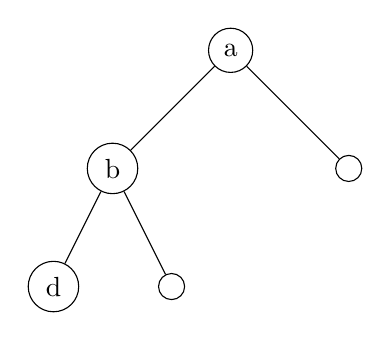
\begin{tikzpicture}[
    every node/.style={circle, draw},
    level/.style={sibling distance=30mm/#1}
  ]
    \node {a}
      child {node {b}
        child {node {d}}
          child {node {}}
      }
      child {node {}
      };
  \end{tikzpicture}
\end{center}

From this graph, $ e(t) = 4 $ and $ b(t) = 3 $

\textbf{Theroem:} For all $ t \in B $, $ e(t) = 1 + b(t) $

We can prove this by structural induction!

\begin{proof}
By structural induction.

\underline{\textbf{Base Case:}}

The number of empty trees in an empty tree is 1. \checkmark

The number of binary trees in an empty tree is 0. \checkmark

\underline{\textbf{Inductive Step:}}

Let $ t_1 $, $ t_2 $ $ \in B $ and suppose $ e(t_1) = 1 + b(t_1) $ and $ e(t_2) = 1 + b(t_2) $.

Then, 
\begin{alignat*}{2}
e( 
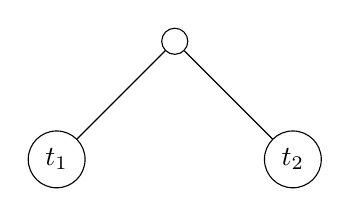
\begin{tikzpicture}[
  every node/.style={circle, draw},
  level/.style={sibling distance=30mm/#1}
]
  \node {}
    child {node {$t_1$}
  }
    child {node {$t_2$}
  };
\end{tikzpicture}
) &=& e(t_1) + e(t_2)
\\
1 + b( 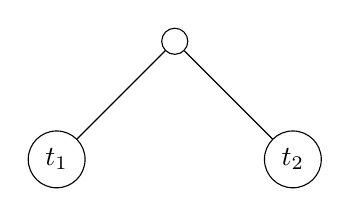
\begin{tikzpicture}[
  every node/.style={circle, draw},
  level/.style={sibling distance=30mm/#1}
]
  \node {}
    child {node {$t_1$}
  }
    child {node {$t_2$}
  };
\end{tikzpicture}
)
&=& 1 + (1 + b(t_1) + b(t_2))
\\
&=& 2 + (b(t_1) + b(t_2))
\\
e(t_1) + e(t_2) &=& (1 + b(t_1)) + (1 + b(t_2)) 
\end{alignat*}
\end{proof}
\clearpage

\section{Combinatorics}
\subsection{Permutations and Combinations}
\textbf{Formulas:}

\begin{alignat*}{2}
  n\;\text{objects, permutate} \;k &= \frac{n!}{(n-k)!} \\
  n\;\text{objects, choose}\; k &= \frac{n!}{k!{(n-k)}!} \\
  n\;\text{categories, permutate} \;k &= n^k 
\end{alignat*}

\subsection{Probability and Expected Value}
Suppose X is a random variable that represents the different outcomes $ x_1, ..., x_n $ with respective
probabilities $p_1, ..., p_n$ then the expected value of X is:

\begin{center}
  $E(X) = p_1x_1 + ... + p_nx_n $
\end{center}

\textbf{Example.} Suppose an algorithm sorts the values in a list and returns the alternating sum/difference 
of the result. For example, if you give it $[5,8,4,1]$ and then sorts to $[1,4,5,8]$ and then returns $1-4+5-8=-6$.

If we are given the following inputs: $[5, 8, 4, 1], [10, 20, 0], [2, 1]\;and\;[0, 5, 2, -3]$.
The following outcomes of each: 
\begin{alignat*}{2}
  [5,8,4,1] &\rightarrow -6\\
  [10,20,0] &\rightarrow -10\\
  [2,1] &\rightarrow -1\\
  [0,5,2,-3] &\rightarrow -1\\
\end{alignat*}
Since all inputs are equally likely, the probability of each input set is $\frac{1}{4}$.
\begin{center}
$0.25(-6) + 0.25(10) + 0.25(-1) + 0.25(-6) = 0.75$
\end{center}
\section{Calculus}
\subsection{Sequences and Sums}
\underline{Some must know sums:}
\begin{alignat*}{2}
  \sum_{i=1}^n 1 &= n \\
  \sum_{i=1}^n i &= \frac{n(n+1)}{2}\\
  \sum_{i=1}^n i^2 &= \frac{n(n+1)(2n+1)}{6}\\
  \sum_{i=0}^n r^i &= \frac{r^{n+1} - 1}{r-1} \\ 
  \sum_{i=0}^n 2^i &= 2^{n+1} - 1\\
  \sum_{i=1}^n i*2^i &= (n-1)2^{n+1} + 2
\end{alignat*}

\textbf{Example:} Let's solve the following sum:
\begin{alignat*}{2}
  \sum_{i=2}^n 2i + 2^{-1}+i^2
\end{alignat*}
First, we split can split the summation up (because of the addition).
\begin{alignat*}{2}
  \sum_{i=2}^n 2i + \sum_{i=2}^n2^{-i} + \sum_{i=2}^ni^2
\end{alignat*}
We can solve each one of these separately now.
\begin{alignat*}{2}
  \sum_{i=2}^n 2i &= 2\sum_{i=2}^n i = 2 \left[\frac{n(n+1)}{2} - 1\right] \\
  \sum_{i=2}^n 2^{-i} &= \sum_{i=2}^n \frac{1}{2}^n = \left[\sum_{i=0}^n \frac{1}{2}^n \right] - 1 
  - \frac{1}{2} = \left[\frac{\frac{1}{2}^{n+1} - 1}{\frac{1}{2}-1}\right] - \frac{1}{2} \\
  \sum_{i=2}^n i^2 &= \frac{n(n+1)(2n+1)}{6} - 1
\end{alignat*}
The results of the sum of those:

\begin{alignat*}{2}
  2\left[\frac{n(n+1)}{2} - 1\right] + \left[\frac{\frac{1}{2}^{n+1} - 1}{\frac{1}{2} -1}\right] - \frac{1}{2} + \left[\frac{n(n+1)(2n+1)}{6}\right] - 1
\end{alignat*}

\subsection{L'hopital Rule}
Things to remeber:

\textbf{Theorem.} Suppose we are trying to evaluate:

\begin{center}
  \[\lim_{x\to\infty}\frac{f(x)}{g(x)}\]
\end{center}
\begin{itemize}
  \item If $\lim_{x\to\infty} f(x)\ = \lim_{x\to\infty} g(x) = 0 $ then:
  \begin{center}
    \[\lim_{x\to\infty}\frac{f(x)}{g(x)} = \lim_{x\to\infty}\frac{f'(x)}{g'(x)} \]

  \end{center}
  \item If $\lim_{x\to\infty} f(x)\ = \lim_{x\to\infty} g(x) = \infty $ then:
  \begin{center}
    \[\lim_{x\to\infty}\frac{f(x)}{g(x)} = \lim_{x\to\infty}\frac{f'(x)}{g'(x)} \]
    
  \end{center}
\end{itemize}
\subsection{Manipulation of Logs}
\begin{alignat*}{2}
  log_b a &= \frac{log_c a}{log_c b} \;\text{(base changes)}\\
  log_b (xy) &= log_b x + log_b y\\
  log_b (\frac{x}{y}) &= log_b{x} - log_b{y}\\
  log_b (x^p) &= p log_b x \\
\end{alignat*}
\end{document}